
\chapter[Bài tập: Quá trình biến đổi lực của con lắc lò xo dao động điều hòa]{Bài tập: Quá trình biến đổi lực của con lắc lò xo dao động điều hòa}
\section{Lý thuyết}
\subsection{Lực đàn hồi}
Độ lớn của lực đàn hồi bằng tích của độ cứng và độ biến dạng của lò xo so với chiều dài tự nhiên.
\begin{equation*} 
	F_\text{đh}=k\left| \Delta l\right|=k\left| l-l_0\right|, 
\end{equation*}
trong đó:
\begin{itemize}
	\item  $k$ là độ cứng của lò xo,
	\item  $\Delta l$ là độ biến dạng của lò xo,
	\item $l$ là chiều dài của lò xo sau khi bị biến dạng,
	\item $l_0$ là chiều dài tự nhiên của lò xo.
\end{itemize}
\subsection{Lực hồi phục (lực kéo về)}
Độ lớn của lực hồi phục bằng tích của độ cứng và li độ của vật.
\begin{equation*} 
	F_\text{hp}=k\left|  x \right|, 
\end{equation*}
trong  đó:
\begin{itemize}
	\item  $k$ là độ cứng của lò xo,
	\item  $x$ là li độ của vật.
\end{itemize}
\section{Mục tiêu bài học - Ví dụ minh họa}
\begin{dang}{Ghi nhớ được công thức tính lực đàn hồi, lực kéo về của con lắc lò xo.}
	
	\viduii{1}{Một con lắc lò xo gồm một vật nhỏ và lò xo nhẹ có độ cứng $k$ dao động điều hòa dọc theo trục O$x$ quanh vị trí cân bằng O. Biểu thức xác định lực kéo về tác dụng lên vật ở li độ $x$ là $F=-kx $. Nếu $F$ tính bằng Niutơn (N), $x$ tính bằng mét (m) thì $k$ tính bằng:
		
		\begin{mcq}(2)
			\item $\text{N}\cdot \text{m}^2$.
			\item $\text{N/m}^2$.
			\item $\text{N}\cdot \text{m}$.
			\item  $\text{N/m}$.
		\end{mcq}	
	}
	{\begin{center}
			\textbf{Hướng dẫn giải}
		\end{center}
		
		Đơn vị của độ cứng $k$ là  $\text{N/m}$.
		
		\textbf{Đáp án: D.}
	}
	\viduii{1}{Trong công thức tính lực đàn hồi của lò xo $F_\text{đh}=k\left| \Delta l\right|$. Đại lượng $\Delta l$ gọi là 
		\begin{mcq}(2)
			\item độ dãn của lò xo.
			\item độ nén của lò xo.
			\item li độ của lò xo.
			\item độ biến dạng của lò xo. 
		\end{mcq}	
	}
	{\begin{center}
			\textbf{Hướng dẫn giải}
		\end{center}
		
		Đại lượng $\Delta l$ gọi là độ biến dạng của lò xo. 
		
		\textbf{Đáp án: D.}
	}
\end{dang}
\begin{dang}{Phân biệt được lực đàn hồi và lực kéo về trong dao động của con lắc lò xo.}
	
	\viduii{2}{Chọn phát biểu đúng.
		
		\begin{mcq}
			\item Đối với con lắc lò xo nằm ngang thì lực kéo về là hợp lực của trọng lực và lực đàn hồi.
			\item Đối với con lắc lò xo thẳng đứng thì lực kéo về là hợp lực của trọng lực và lực đàn hồi.
			\item  Đối với con lắc lò xo nằm ngang thì lực kéo về không phải là lực đàn hồi.
			\item  Đối với con lắc lò xo thẳng đứng thì lực kéo về là lực đàn hồi.
		\end{mcq}	
	}
	{\begin{center}
			\textbf{Hướng dẫn giải}
		\end{center}
		
		Đối với con lắc lò xo thẳng đứng thì lực kéo về là hợp lực của trọng lực và lực đàn hồi.
		
		\textbf{Đáp án: B.}
	}
	\viduii{2}{Chọn chiều dương thẳng đứng, hướng xuống dưới, gốc tọa độ tại vị trí cân bằng. Trong một chu kỳ của con lắc lò xo treo thẳng đứng, lực kéo về và lực đàn hồi
		\begin{mcq}
			\item cùng chiều nhau khi vật có li độ âm. 
			\item cùng chiều nhau khi vật có li độ dương. 
			\item ngược chiều nhau khi vật có li độ dương. 
			\item ngược chiều nhau khi vật có li độ âm.  
		\end{mcq}	
	}
	{\begin{center}
			\textbf{Hướng dẫn giải}
		\end{center}
		
		Chọn chiều dương thẳng đứng, hướng xuống dưới, gốc tọa độ tại vị trí cân bằng. Trong một chu kỳ của con lắc lò xo treo thẳng đứng, lực kéo về và lực đàn hồi cùng chiều nhau khi vật có li độ dương. 
		
		\textbf{Đáp án: B.}
	}
\end{dang}
\begin{dang}{ Xác định được lực đàn hồi và chiều dài của con lắc lò xo khi đặt nằm ngang và thẳng đứng}
	\ppgiai{
		
		\begin{enumerate} 
			\item Lực đàn hồi $F_\text{đh}=k|\Delta l|$.
			\begin{itemize}
				\item Khi con lắc lò xo nằm ngang: $\Delta l=|x|$.
				
				Do đó, độ lớn lực đàn hồi $F_\text{đh(max)}=kA$ ở hai biên, $F_\text{đh(min)}=0$ ở vị trí cân bằng.
				
				\item Khi con lắc lò xo thẳng đứng:	$\Delta l=|\Delta l_0 +x|$, trong đó $\Delta l_0$ là độ biến dạng của lò xo ở vị trí cân bằng, chiều dương thẳng đứng hướng xuống dưới.
				
				Do đó:
				\begin{itemize}
					\item	lực đàn hồi cực đại $F_\text{đh(max)}=k\left(\Delta l_0 + A\right) $ khi vật ở biên dương.
					\item 	lực đàn hồi cực tiểu $F_\text{đh(min)}=k\left(\Delta l_0 - A\right) $ khi $A<\Delta l_0$ và vật ở biên âm.
					\item 	lực đàn hồi cực tiểu $F_\text{đh(min)}=0$ khi $A>\Delta l_0$ khi vật ở vị trí lò xo không bị biến dạng.
				\end{itemize}
				
			\end{itemize}
			
			\item Chiều dài con lắc lò xo.
			
			\begin{itemize}
				\item Khi con lắc lò xo nằm ngang: $l=l_0+ x$, với $l_0$ là chiều dài tự nhiên của lò xo, chiều dương hướng ra xa điểm treo. 
				
				Do đó, chiều dài lớn nhất lò xo $l_\text{max}=l_0+A$, $l_\text{min}=l_0-A$.
				
				\item Khi con lắc lò xo thẳng đứng:	$l=l_\text{CB}+x$, trong đó $\Delta l_\text{CB}=l_0+\Delta l_0$ là chiều dài của lò xo ở vị trí cân bằng, chiều dương thẳng đứng hướng xuống dưới.
				
				Do đó:
				\begin{itemize}
					\item	chiều dài cực đại $l_\text{max}=l_\text{CB}+A $ (ở biên dương).
					\item  chiều dài cực đại $l_\text{min}=l_\text{CB}-A $ (ở biên âm).
				\end{itemize}
				
				\item Công thức tính: $l_\text{CB}=\dfrac{l_\text{max}+l_\text{min}}{2}, \ A=\dfrac{l_\text{max}-l_\text{min}}{2}$
				
			\end{itemize}
			
			
		\end{enumerate} 
		
	}
	
	
	\viduii{3}{	Một con lắc lò xo có chiều dài tự nhiên $l_0 = \SI{30}{cm}$, độ cứng của lò xo  là $k=10\ \text{N/m}$. Treo vật nặng có khối lượng 0,1 kg vào lò xo và kích thích cho lò xo dao động điều hòa theo phương thẳng đứng với biên độ $A=\SI{5}{cm}$. Xác định chiều dài cực đại, cực tiểu của lò xo trong quá trình dao động của vật.
		\begin{mcq}(2)
			\item 40 cm; 30 cm.
			\item 45 cm; 25 cm.
			\item 35 cm; 55 cm.
			\item 45 cm; 35 cm.
		\end{mcq}
		
	}
	{\begin{center}
			\textbf{Hướng dẫn giải}
		\end{center}
		Ta có: $l_0 = \SI{30}{cm}$ và $\Delta l_0 =\dfrac{mg}{k} = \SI{10}{cm}$ và $l_\text{max} = l_0 +\Delta l_0 + A =\SI{45}{cm}$. 
		
		$l_\text{min} = l_0+\Delta l_0 -A = \SI{35}{cm}$.
		
		\textbf{Đáp án: D.}
	}
	\viduii{3}{	Một con lắc lò xo có chiều dài tự nhiên $l_0 =\SI{30}{cm}$, độ cứng của lò xo là $k=10\ \text{N/m}$. Treo vật nặng có khối lượng 0,1 kg vào lò xo và kích thích lò xo dao động điều hòa theo phương thẳng đứng với biên độ $A=\SI{20}{cm}$. Xác định lực đàn hồi cực đại, cực tiểu của lò xo trong quá trình dao động của vật.
		
		\begin{mcq}(2)
			\item 1,5 N; 0 N.
			\item 2 N; 0 N.
			\item 3 N; 0 N.
			\item Không đáp án.
		\end{mcq}
	}
	{\begin{center}
			\textbf{Hướng dẫn giải}
		\end{center}
		
		Ta có $\Delta l_0 = \SI{0,1}{m} <A$ nên $F_{\text{đh}_\text{max}} = k(A+\Delta l_0) = \SI{3}{N}.$
		
		và $F_{\text{đh}_\text{min}} =0 $ vì $\Delta l_0<A$.
		
		\textbf{Đáp án: C.}
	}
	
	
\end{dang}


\begin{dang}{Sử dụng được đường tròn lượng giác,\\ công thức xác định lực đàn hồi, lực kéo về để xác định thời gian nén dãn của con lắc lò xo.
	}
	\ppgiai{
		
		\begin{center}
			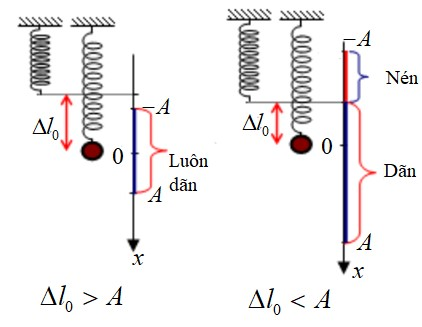
\includegraphics[scale=0.7]{../figs/VN12-PH-03-A-002-2-V2-1.jpg}
		\end{center}
		\begin{itemize}
			\item Khi $\Delta l_0>A$ thì lò xo luôn dãn nên thời gian dãn bằng chu kỳ dao động $T$, thời gian nén bằng 0.
			
			\item Khi $\Delta l_0<A$:
			\begin{center}
				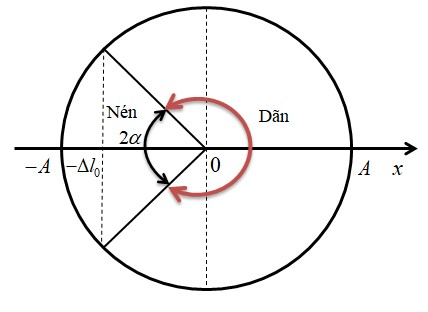
\includegraphics[scale=0.7]{../figs/VN12-PH-03-A-002-2-V2-2.jpg}
			\end{center}
			\begin{equation*} 
				\varphi_\text{nén}=2\alpha,
			\end{equation*}
			với $\alpha$ được tính bởi công thức:
			
			\begin{equation*} 
				\cos \alpha=\dfrac{\Delta l_0}{A}\Rightarrow \alpha=\arccos \dfrac{\Delta l_0}{A},
			\end{equation*}
			trong đó, $\Delta l_0$ là độ biến dạng của lò xo khi vật ở vị trí cân bằng, $A$ là biên độ.
			
			Thời gian lò xo nén trong một chu kỳ là
			\begin{equation*} 
				t_\text{nén}=\dfrac{\varphi_\text{nén}}{\omega}=2\cdot \dfrac{\arccos \dfrac{\Delta l_0}{A}}{\omega},
			\end{equation*}
			
			Thời gian lò xo dãn trong một chu kỳ là
			\begin{equation*} 
				t_\text{dãn}=\dfrac{\varphi_\text{dãn}}{\omega}=\dfrac{2\pi-\varphi_\text{nén}}{\omega}=T-t_\text{nén}.
			\end{equation*}
			
			
			
		\end{itemize}
		
		
	}
	
	\viduii{3}{Con lắc lò xo treo thẳng đứng, độ cứng $k=50\ \text{N/m}$, vật nặng khối lượng $m = 200\ \text{g}$ dao động điều hòa  theo phương thẳng đứng với biên độ $A =4\sqrt{2}\ \text{cm}$, lấy $g =\pi^2= 10\ \text{m/s}^2$.  Trong   một chu kỳ, thì thời gian lò xo nén bằng 
		\begin{mcq}(4)
			\item  $\text{0,2}\ \text{s}$.
			\item  $\text{0,1}\ \text{s}$.
			\item $\text{0,3}\ \text{s}$.
			\item $\text{0,5}\ \text{s}$.
		\end{mcq}
	}
	{\begin{center}
			\textbf{Hướng dẫn giải}
		\end{center}
		
		$\omega=\sqrt{\dfrac{k}{m}}=4\pi\ \text{rad/s}$.
		
		Tần số góc $\omega=\sqrt{\dfrac{k}{m}}=5\pi\ \text{rad/s}$.
		
		Độ biến dạng của lò xo khi vật ở vị trí cân bằng $\Delta l_0=\dfrac{g}{\omega^2}=\text{4}\ \text{cm}$.
		
		$\cos \alpha=\dfrac{\Delta l_0}{A}\Rightarrow \alpha=\arccos \dfrac{\Delta l_0}{A}=\dfrac{\pi}{4}$.
		
		Thời gian lò xo nén là $t_\text{nén}=\dfrac{\varphi_\text{nén}}{\omega}=\dfrac{2\alpha}{\omega}=\text{0,1}\ \text{s}$.
		
		\textbf{Đáp án: B.}
	}
	\viduii{3}{Một con lắc lò xo dao động treo thẳng đứng khi cân bằng lò xo dãn 3 cm. Bỏ qua mọi lực cản. Kích thích cho vật dao động điều hòa theo phương thẳng đứng thì thấy thời gian lò xo bị nén trong một chu kỳ là $\dfrac{T}{3}$ ($T$ là chu kỳ dao động của vật). Lấy $g =\pi^2= 10\ \text{m/s}^2$. Biên độ dao động $A$ của  vật nặng bằng
		\begin{mcq}(4)
			\item  $\text{6}\ \text{cm}$.
			\item  $\text{3}\ \text{cm}$.
			\item $\text{4}\ \text{cm}$.
			\item $\text{5}\ \text{cm}$.
		\end{mcq}
	}
	{\begin{center}
			\textbf{Hướng dẫn giải}
		\end{center}
		
		Khi vật ở vị trí cân bằng thì lò xo dãn một đoạn $\Delta l_0=3\ \text{cm}$.
		
		
		Thời gian lò xo nén trong một chu kỳ là $\dfrac{T}{3}$ nên:
		
		$t_\text{nén}=\dfrac{\varphi_\text{nén}}{\omega}=\dfrac{\varphi_\text{nén}}{2\pi/T}=\dfrac{T}{3}$.
		
		$\Rightarrow \varphi_\text{nén}=\dfrac{2\pi}{3}\Rightarrow \alpha=\dfrac{\pi}{3}$.
		
		$\cos \alpha=\dfrac{\Delta l_0}{A}=\cos \dfrac{\pi}{3}=\dfrac{1}{2}$.
		
		$\Rightarrow A= 2\Delta l_0=\text{6}\ \text{cm}$.
		
		\textbf{Đáp án: A.}
	}
	
	
\end{dang}
